\documentclass[tikz,border=8pt]{standalone}
% Shared look for every TikZ diagram. Load with % Shared look for every TikZ diagram. Load with % Shared look for every TikZ diagram. Load with \input{../../tools/tikz-style.tex}
\usepackage[T1]{fontenc}
\usepackage{lmodern}
\renewcommand{\sfdefault}{lmr}  % diagrams use the same serif as the text
\usetikzlibrary{arrows.meta, positioning, shapes.geometric, calc, fit, backgrounds}
\definecolor{cblue}{HTML}{4C78A8}
\definecolor{corange}{HTML}{F58518}
\definecolor{cgreen}{HTML}{54A24B}
\definecolor{cred}{HTML}{E45756}
\definecolor{cpurple}{HTML}{B279A2}
\definecolor{cgrey}{HTML}{6B6B6B}
\tikzset{
  every picture/.style={font=\sffamily, line width=1.2pt},
  box/.style={draw=#1, fill=#1!12, rounded corners=4pt, align=center, inner sep=7pt, minimum height=1.1cm},
  box/.default=cgrey,
  arrow/.style={-{Stealth[length=3mm]}, draw=cgrey, line width=1.4pt},
  title/.style={font=\sffamily\bfseries\Large},
  note/.style={font=\sffamily\small, text=cgrey, align=center},
}
\AtBeginDocument{\hyphenpenalty=10000 \exhyphenpenalty=10000}

\usepackage[T1]{fontenc}
\usepackage{lmodern}
\renewcommand{\sfdefault}{lmr}  % diagrams use the same serif as the text
\usetikzlibrary{arrows.meta, positioning, shapes.geometric, calc, fit, backgrounds}
\definecolor{cblue}{HTML}{4C78A8}
\definecolor{corange}{HTML}{F58518}
\definecolor{cgreen}{HTML}{54A24B}
\definecolor{cred}{HTML}{E45756}
\definecolor{cpurple}{HTML}{B279A2}
\definecolor{cgrey}{HTML}{6B6B6B}
\tikzset{
  every picture/.style={font=\sffamily, line width=1.2pt},
  box/.style={draw=#1, fill=#1!12, rounded corners=4pt, align=center, inner sep=7pt, minimum height=1.1cm},
  box/.default=cgrey,
  arrow/.style={-{Stealth[length=3mm]}, draw=cgrey, line width=1.4pt},
  title/.style={font=\sffamily\bfseries\Large},
  note/.style={font=\sffamily\small, text=cgrey, align=center},
}
\AtBeginDocument{\hyphenpenalty=10000 \exhyphenpenalty=10000}

\usepackage[T1]{fontenc}
\usepackage{lmodern}
\renewcommand{\sfdefault}{lmr}  % diagrams use the same serif as the text
\usetikzlibrary{arrows.meta, positioning, shapes.geometric, calc, fit, backgrounds}
\definecolor{cblue}{HTML}{4C78A8}
\definecolor{corange}{HTML}{F58518}
\definecolor{cgreen}{HTML}{54A24B}
\definecolor{cred}{HTML}{E45756}
\definecolor{cpurple}{HTML}{B279A2}
\definecolor{cgrey}{HTML}{6B6B6B}
\tikzset{
  every picture/.style={font=\sffamily, line width=1.2pt},
  box/.style={draw=#1, fill=#1!12, rounded corners=4pt, align=center, inner sep=7pt, minimum height=1.1cm},
  box/.default=cgrey,
  arrow/.style={-{Stealth[length=3mm]}, draw=cgrey, line width=1.4pt},
  title/.style={font=\sffamily\bfseries\Large},
  note/.style={font=\sffamily\small, text=cgrey, align=center},
}
\AtBeginDocument{\hyphenpenalty=10000 \exhyphenpenalty=10000}

\begin{document}
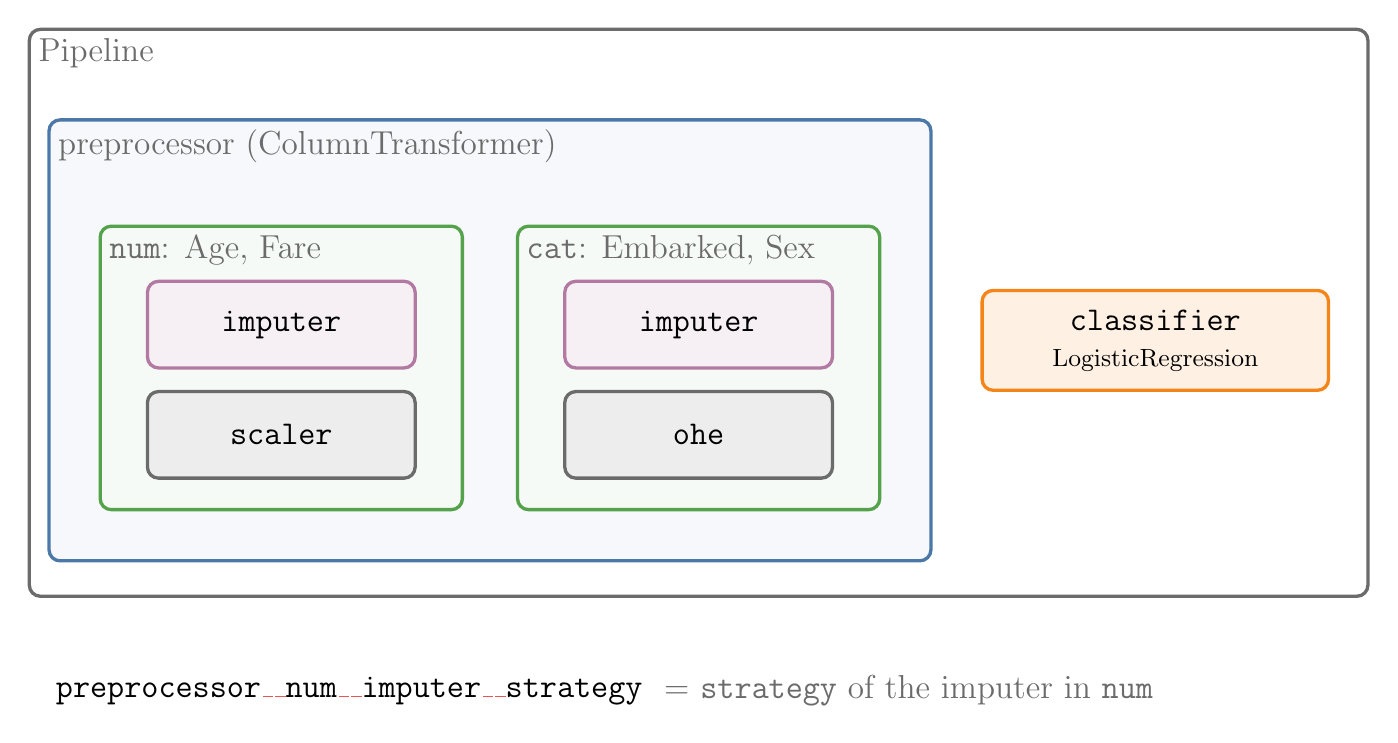
\begin{tikzpicture}[
    step/.style={box=#1, minimum width=3.3cm, font=\large\ttfamily}, every node/.append style={font=\large},
    note/.style={font=\large, text=cgrey, align=center}]
  % the nested pipeline, each box labelled with its step name
  \node[step=cgrey, minimum width=17cm, minimum height=7.2cm, fill=white] (pipe) at (6.5,-2.4) {};
  \node[note, anchor=north west] at (pipe.north west) {Pipeline};
  \node[step=cblue, minimum width=11.2cm, minimum height=5.6cm, fill=cblue!5] (pre) at (3.85,-2.75) {};
  \node[note, anchor=north west] at (pre.north west) {preprocessor (ColumnTransformer)};
  \node[step=corange, minimum width=4.4cm, minimum height=0.9cm] (cls) at (12.3,-2.75) {classifier\\[-1pt]\normalfont\small LogisticRegression};
  % the two inner pipelines
  \newcommand{\inner}[5]{% #1 name, #2 x, #3 columns, #4 second step
    \node[step=cgreen, minimum width=4.6cm, minimum height=3.6cm, fill=cgreen!5] (#1) at (#2,-3.1) {};
    \node[note, anchor=north west] at (#1.north west) {\texttt{#1}: #3};
    \node[step=cpurple, minimum width=3.4cm] at (#2,-2.55) {imputer};
    \node[step=cgrey, minimum width=3.4cm] at (#2,-3.95) {#4};
  }
  \inner{num}{1.2}{Age, Fare}{scaler}{}
  \inner{cat}{6.5}{Embarked, Sex}{ohe}{}
  % how the names join up
  \node[font=\ttfamily\large, anchor=west] (path) at (-1.8,-7.2)
    {preprocessor\textcolor{cred}{\_\_}num\textcolor{cred}{\_\_}imputer\textcolor{cred}{\_\_}strategy};
  \node[note, anchor=west] at (path.east) {= \texttt{strategy} of the imputer in \texttt{num}};
\end{tikzpicture}
\end{document}
